\chapter{Results and Discussion}

\section{Piezo1 as integrator of biomechanical events}
Piezo1 has been established as important mechanotransductive element \cite{Murthy2017PiezosTU} \myworries{Two Papers from Mendeley} in a plethora of different physiological contexts. Here we address the issue of transferability and try to determine, whether Piezo1 is equally important in the mechanosensing by mesenchymal stem cells.\\
For each biological replicates we have at least 3 different flowchambers as technical replicates. Reasons for possible exclusion of a measurement were either movement artefacts in between measurements or the compromised integrity of the flowchamber at hand. Segmentation was done once per sample at the beginning. After image processing, all samples from the same donor were pooled. The protocol of the calcium imaging can be found \myworries{Where?}\\

\subsection{MSC's and shear}
Making use of in-house developed flowchambers, we measured an increase of maximal relative fluorescence levels directly relating to shear stress. This supports the notion of calcium influx as immediate reaction to shear in mesenchymal stem cells, similar to what we would expect in tendon. Follow up experiments with two Piezo1 knock-out cell lines (P1-395, P1-555) indicated that Piezo1 is the main trigger, as calcium-response was largely lacking when compared to negative control (No Target KO Cell line) \\ \myworries{Insert Fabian's graph with KO Cell lines}

\subsection{Functionalization of Medium}
The insight from before relies on the assumption of the calcium-ion-influx being a primary consequence of Piezo1 opening, as opposed by the hypothesis that activate Piezo1 channels might elicit a secondary reaction, like release of ionic calcium that is stored in the endoplasmatic reticulum. To test this assumption, we designed an experiment, with the medium as the experimental condition.\\
Flushing the same flowchamber twice, one time with calcium-free ACSF and another time with normal ACSF, we saw an average of 40\% increase in measured $F_{max}/F_{0}$ levels in the second measurement, without a detectable signal during the Calcium-free Measurement ($n=3$ biological replicates).\par

To conclude, this result combined with the results from before shows that not only do MSC also feel shear stress, but the associated extracellular calcium ion influx is \Piezo mediated. 

\subsection{Caveats}
The main assumptions that deserve special mention are twofold: The Shear Protocol and the Protocol to increase cellular adherence. \par

\textsc{Shear protocol}\\
a. physiological context. Fluidic shear more likely to simluate endothelial blood interplay.\\
a. Viscosity? Turbulences etc.\\
\textsc{Adherence}\\
a. Sulfo-SANPAH known to modify substrate stiffness with possible consequences for cells\\
a. Collagen is not sufficient to simulate the whole ECM. Likely we are missing some important mediators.

\section{Piezo1 and the extracellular matrix}

Preliminary mass spectroscopy secretome analysis of \Yoda-treated cells showed a distinct decrease in core extracellular matrix (ECM) components, such as alpha-1 type I collagen(\colone), Fibronectin-1 (\textsc{Fn1}) and finally alpha-1 type III collagen (\colthree).
This inspired further investigation into this matter.\par

The experiment was set up to allow for both Protein Analysis (i.e. Western Blot) and mRNA-concentration Analysis (i.e. qRT-PCR) of identical samples.\\
By measures of SDS-PAGE, we were able to compare intracellular protein content of \Yoda-treated cells with control. There we saw a \myworries{very sharp} decline in \colone-content, which corroborate the findings from the secretome analysis \myworries{Input Figure Reference}. Surprisingly, the effects were not only marked by fast onset but also of long-lasting nature, since the effect of a singular 30 minutes \Yoda-exposition remained the same three days after intervention. This supports the notion of the involvement of Piezo1-Activation in ECM-homeostasis in MSC's. \par

We see three possible explanations, while not excluding any combination thereof: The first and most straightforward explanation involves an change in cellular dynamics somewhere between transcription and translation, resulting in a \textit{de facto} decrease in protein synthesis. Naturally, increased catabolic activity could also be the explanation. Finally, the third possible explanation would be a stronger secretion to the interstitial space, thus decreasing intracellular protein levels. The third explanation is contradicted by the inital secretome analysis, which shows a decrease also in amount of secreted protein.

In parallel, we also looked at mRNA representation through qRT-PCR, where we biased our analysis towards \colone{ }, \colthree{ }, \textsc{Fn}1 
and Interleukin-6 to confirm our prior results.  All measurements were normalised against negative control samples which where harvested immediately after the intervention ended.\\
While we were not able to produce a significant result in any time point or gene, we saw a tendency of decreasing \colone. Sadly, due to time constrictions related to the duration of this thesis, we were not able to produce more data points. It is likely to produce a significant result with increasing sample size. On the other hand, the RNA levels diverged reproducibly from identical protein samples.

This discrepancy between Protein and mRNA is especially curious, when considering the natural sequence of Gene $>$ RNA $>$ Protein, after a transcriptional change. Intuitively, mRNA precedes Protein, meaning a change in transcription would first be seen in RNA levels, with Protein lagging behind, 
something to consider in knock-out studies. However, it seems to not be given here. While some adaptation on mRNA-levels could also happen (look at:  \colone), the clear finding from the Western Blots is remarkably not translated in RNA. The assumption often made in other works,\myworries{Insert other sources that do this.} that RNA and protein are congruent is heavily violated here. qRT-PCR analysis adds evidence that speaks against the degradation of RNA as explanation for the effect seen in Protein analysis. 

This result is both unexpected and intriguing. The divergence between results from Western Blot and qRT-PCR introduces a new dimension, inspiring further research into the topic. With Piezo1-induced protein degradation being a possible explanation, we can start formulating testable hypothesis, like identifying possibly involved 

\begin{itemize}
     \item  Caveat: Likely differentiation during experiment. FGF-2 (fibroblast growth factor, known for suppressing ECM-production \myworries{[citation needed]}) not present during experiment, but during whole cell culture. Same thing with FBS. 
     
     \item Maybe Calcium itself leads to degradation
    
    \item Reversibility experiment shows lacking recovery from Yoda-stimulus. Even when FBS is administered after 3-day period.
\end{itemize}



\begin{figure}[ht]
    \centering
    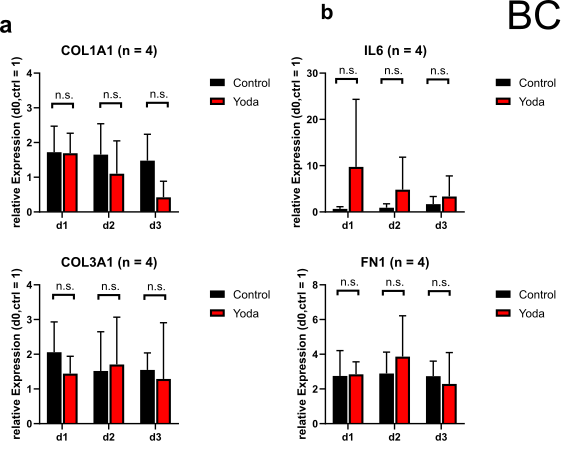
\includegraphics[scale = 0.6]{Collection.png}
    \caption{
    PCR Experiments where we saw some really cool stuff happening.
    \textbf{a}: \colone{ }
    \textbf{b}: Interleukin 6
    \textbf{c}: \colthree{ }
    \textbf{d}: \textsc{Fn}1
    All Experiments were n = 4. 
    }
    \label{fig:my_label}
\end{figure}

\section{Piezo1 and osteogenic differentiation}
Here I'm basically going to mention that due to long-term nature of the effect we suspected differentiation. Since Proteins investigated are heavily implicated with Osteogenic differentiation, we looked into osteogenic differentiation. Enter Graph. Even though some tendency can be seen, results of those markers are not significant. 


\section{Excursion: Biostability of Yoda1 and Piezo1 mediated apoptosis}
\label{sec:biostability}
Curious case of Yoda1 loosing its effect completey after only 8h incubation. Also we reproducibly have seen that cells die after Yoda1 stimulation. Uli made some experiments with KO's that showed no decrease in cell viability even after Yoda1-treatment. Some pictures I can add here